\section{Testowanie aplikacji}

W celu sprawdzenia poprawności działania aplikacji wykonano 2 rodzaje testów:

\begin{itemize}
	\item Testy funcjonalne
	\item Wykorzystanie algorytmu do grupowania pikseli na bitmapach
\end{itemize}

Pierwszy z nich został wykonany w celu sprawdzenia poprawności zaimplementowanego rozwiązania. Drugi rodzaj testów posłużył do zaprezentowania przykładowych wyników, jakie można uzyskać posługując się algorytmem k-średnich.

\subsection{Testy funkcjonalne}

Testy funkcjonalne wykoanano na dwóch typach danych: reprezentującym liczby całkowite i wbudowany w język C++ typ \texttt{int} oraz własnej klasie \texttt{Point\textunderscore 2D} reprezentującej punkt w przestrzeni euklidesowej. Na czas testów flaga \texttt{printOutput} ustawiona została na wartość \texttt{true}.

Na rysunku \ref{img:intTest} zaprezentowano i omówiono kolejne kroki wywołania dla typu całkowitego. Wykonano podział na 3 grupy, a warunkiem stopu był stan stabilny.

\begin{enumerate}
	\item Przed pierwszą iteracją w sposób losowy wybrano wartości centroidów pośród elementów początkowych. Wybór padł na wartości 0, 9 oraz 10.
	\item W pierwszej iteracji wpierw przypisano dane do grup na podstawie odległości od centroidów. Miarą odległości była wartość dzieląca obie liczby na osi X. Liczby 0, 9 oraz 10 jako środki grup zostały automatycznie przypisane do grup kolejno 0, 1 oraz 2. Pozostałe elementy najbliżej położone były wartości 0, więc przypisano je do grupy numer 0. Następnie wyliczono nowe wartości centroidów -- grupy 1 oraz 2 zawierały tylko po jednym elemencie, więc ich wartość nie uległa zmianie. Nowa wartość centroidu grupy zerowej obliczona została za pomocą średniej arytmetycznej z 6 należących do niej elementów i jest równa -2.
	\item W iteracji drugiej iteracji można zaobserwować, że element o indeksie 3 (i wartości 4) jest bliżej położony środka grupy pierwszej (odległość wynosi 5) niż zerowej (odległość równa 6), więc w tej iteracji zmienia skupienie na numer 1. W ten sposób zmianie ulegają skupienia 0 i 1, dlatego następuje przesunięcie współrzędnych ich środków (na kolejno -3 i 6).
	\item W iteracji trzeciej można zaobserwować migrację elementu o indeksie 0 do grupy pierwszej oraz elementu o indeksie 7 do grupy 2. Ponieważ wartości centroidów są tego samego typu co elementy wejściowe, ich wartość po ponownym obliczeniu jest zaokrąglana w dół.
	\item Iteracja czwarta -- element o indeksie 4 (wartość 0) zmienia grupę na pierwszą, gdyż bliżej mu do wartości 3 niż -5. Na nowo obliczane są środki skupień grup 0 i 1.
	\item W iteracji piątej nie ma przejść elementów między grupami -- osiągnięto stan stabilny, dalsze iteracje nie są potrzebne.
	\item Na końcu następuje grupowanie oraz wyznaczenie elementów zwracanych -- na początek zakresu przesuwane są elementy należące do grupy zerowej: -5, -6 i -9. W następnej kolejności znajdują się dane należące do pierwszego skupienia, czyli 4, 0 i 3. Na końcu znajdują się elementy grupy drugiej -- 10 oraz 9. Wektor zwracany zawiera iteratory wskazujące na na indeksy 0, 3 oraz 6 (początki kolejnych grup).
\end{enumerate}

\begin{figure}[!h]
	\centering
	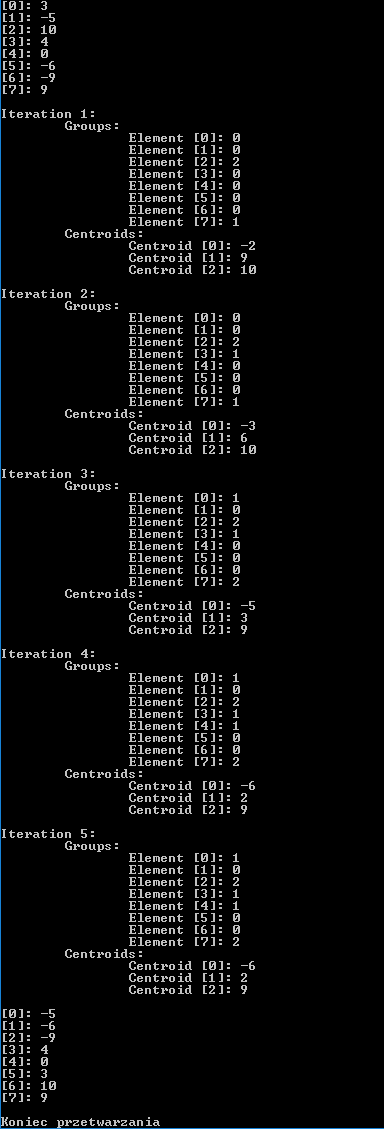
\includegraphics[width=0.40\textwidth]{./img/intTest.png}
	\caption{Przykładowe wywołanie algorytmu dla zmiennych typu całkowitego}
	\label{img:intTest}
\end{figure}

\subsection{Grupowanie pikseli}

Testy praktyczne wykonane zostały na bitmapach przygotowanych własnoręcznie lub pobranych z Internetu. Testy te pozwalają prześledzić zachowanie algorytmu. W tym celu skorzystanego z biblioteki zewnętrznej dostępnej pod adresem \url{http://partow.net/programming/bitmap/index.html}. W trakcie wczytywania danych (współrzędnych pikseli) pomijano piksele białe (o wartości RGB równej FFFFFF).

\subsubsection{Zależność od warunku stopu}

\begin{figure}[!h]
	\centering
	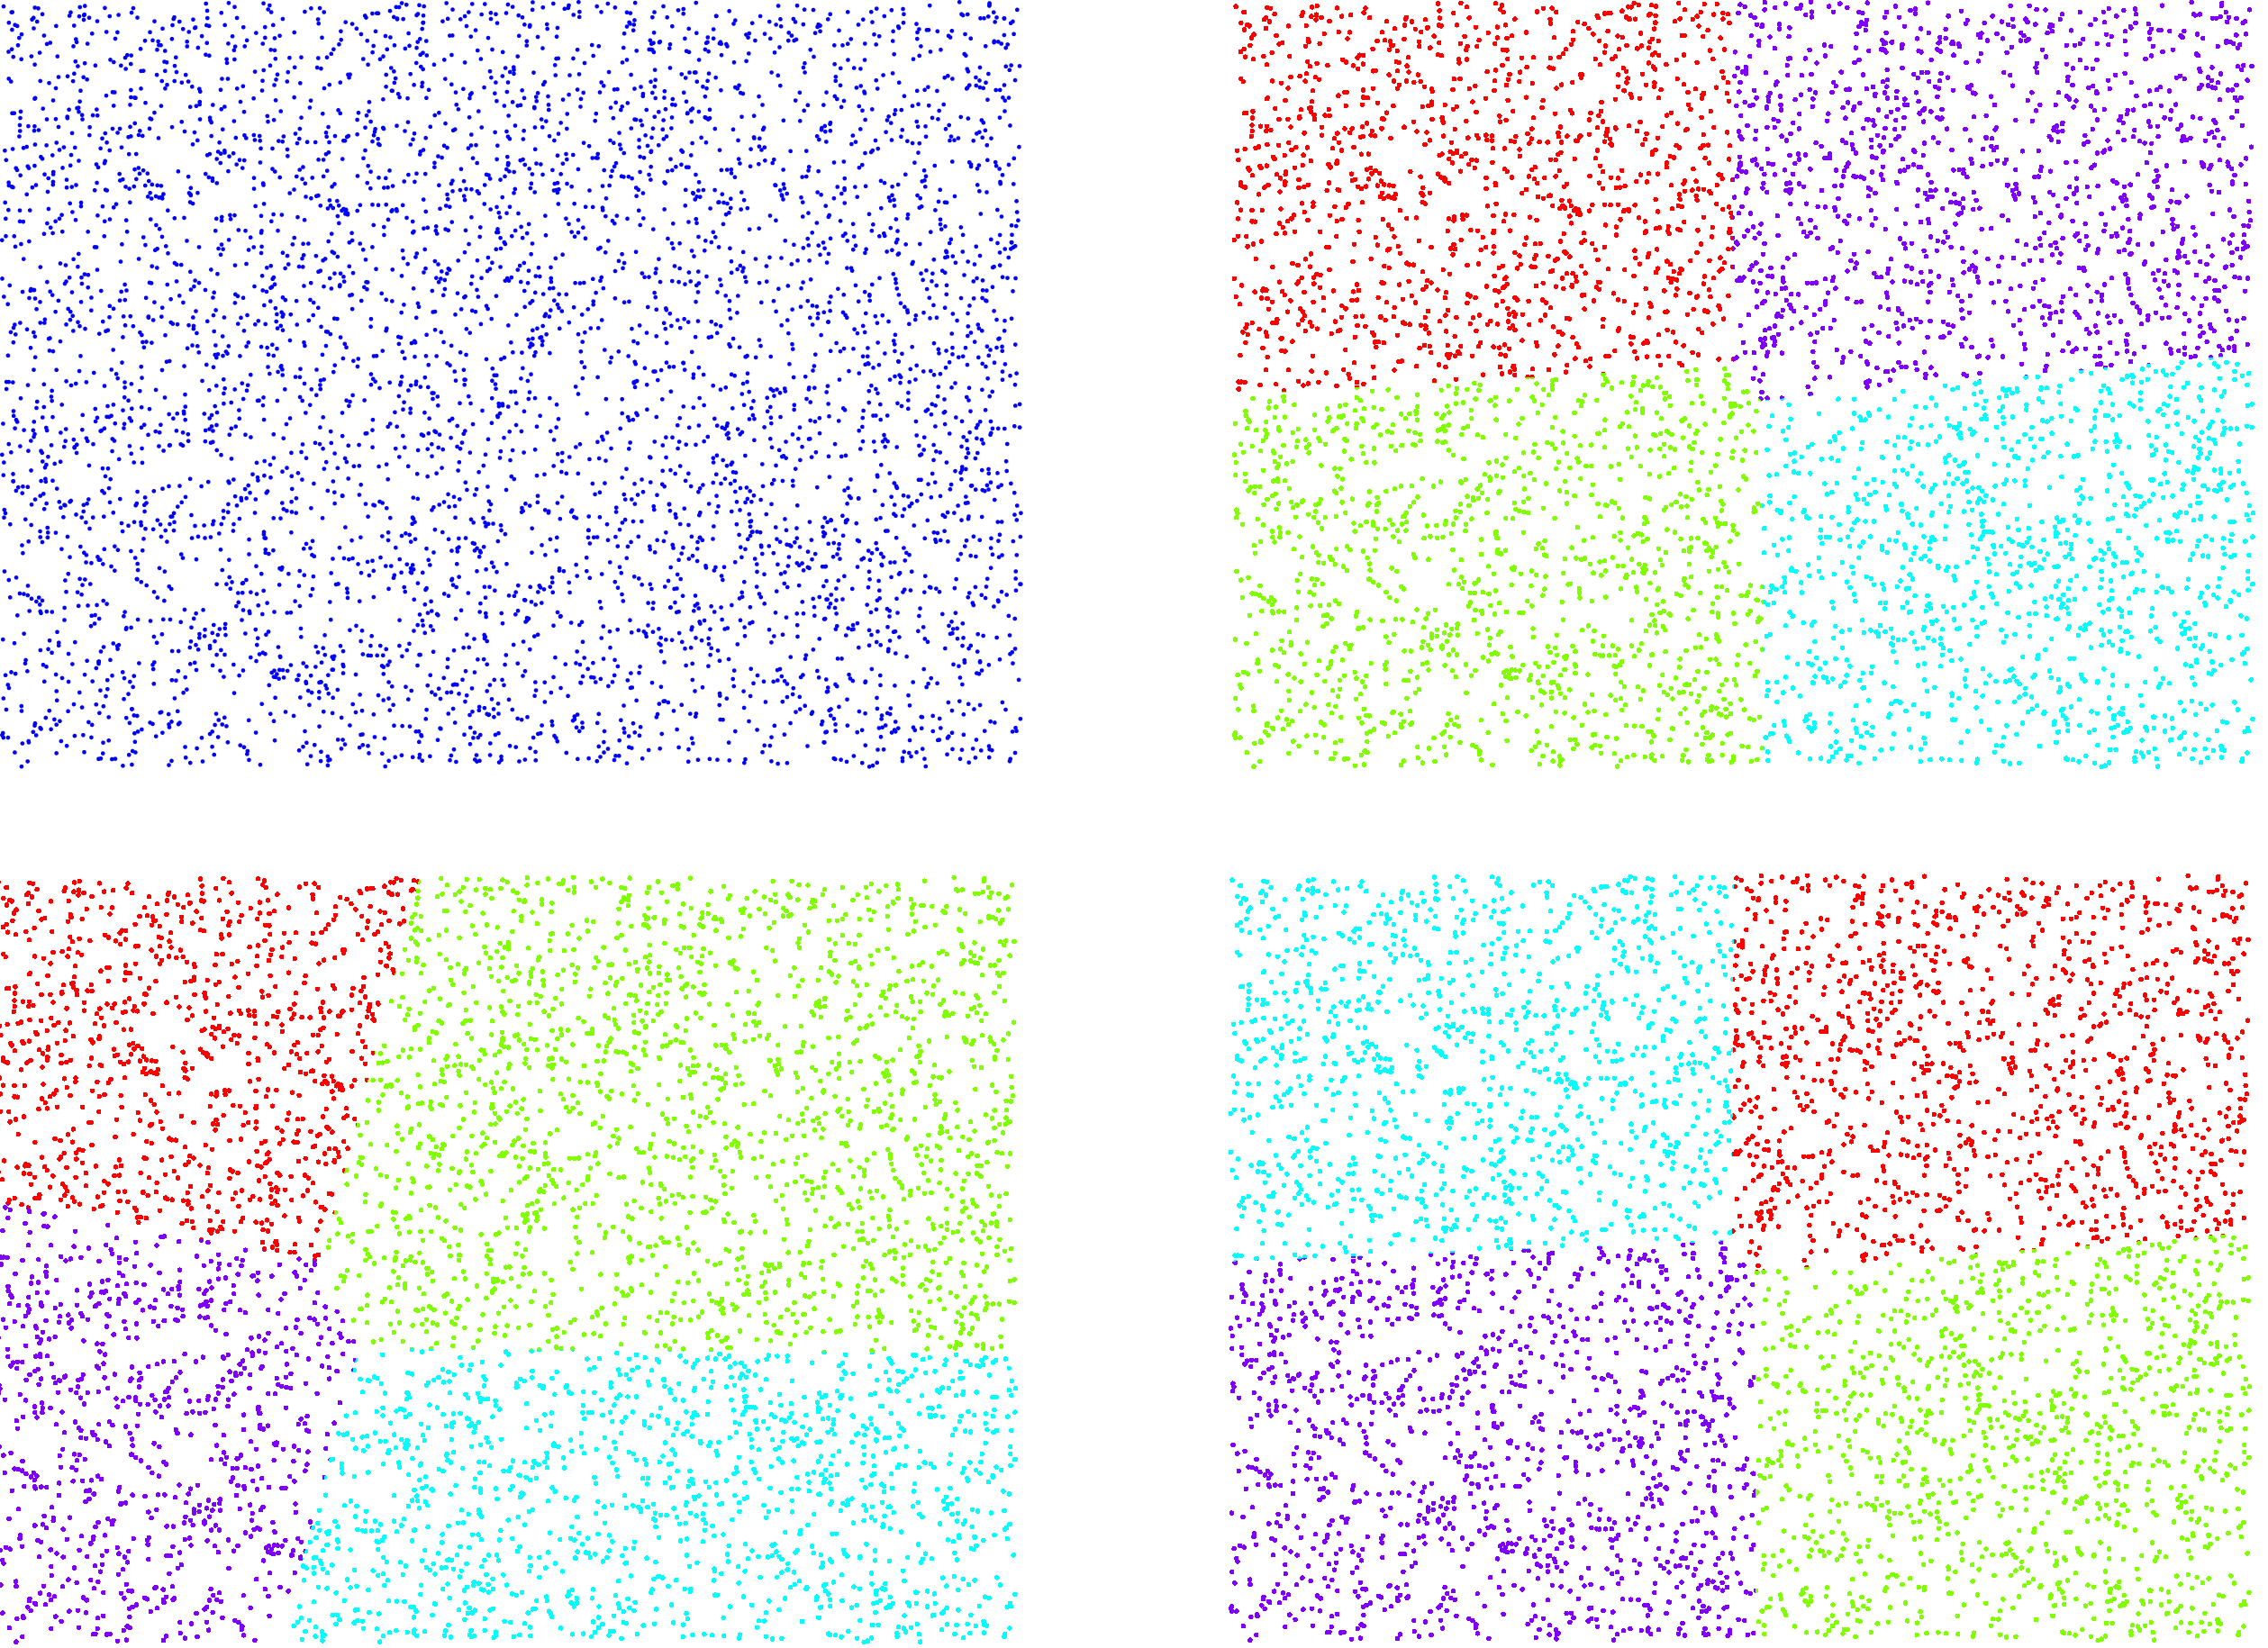
\includegraphics[width=0.7\textwidth]{./img/condition.png}
	\caption{Od górnego lewego rogu zgodnie ze wskazówkami zegara: obraz oryginalny, stan stabilny, liczba iteracji = 10, liczba iteracji = 2}
	\label{img:cond}
\end{figure}

Na rysunku nr \ref{img:cond} przedstawiono wyniki wykonania algorytmu dla różnych warunków stopu. Liczbę grup ustawiono na 4. Można zaobserwować fakt, że dla małej liczby iteracji algorytm nie zdążył jeszcze ustabilizować wyników i dla w miarę równomiernego rozkładu danych na płaszczyźnie grupy są bardzo nierówne. Dla większej liczby iteracji (10) wynik jest zbliżony do tego otrzymanego poprzez wybranie stanu stabilnego.

\subsubsection{Zależność od liczby grup}

\begin{figure}[!h]
	\centering
	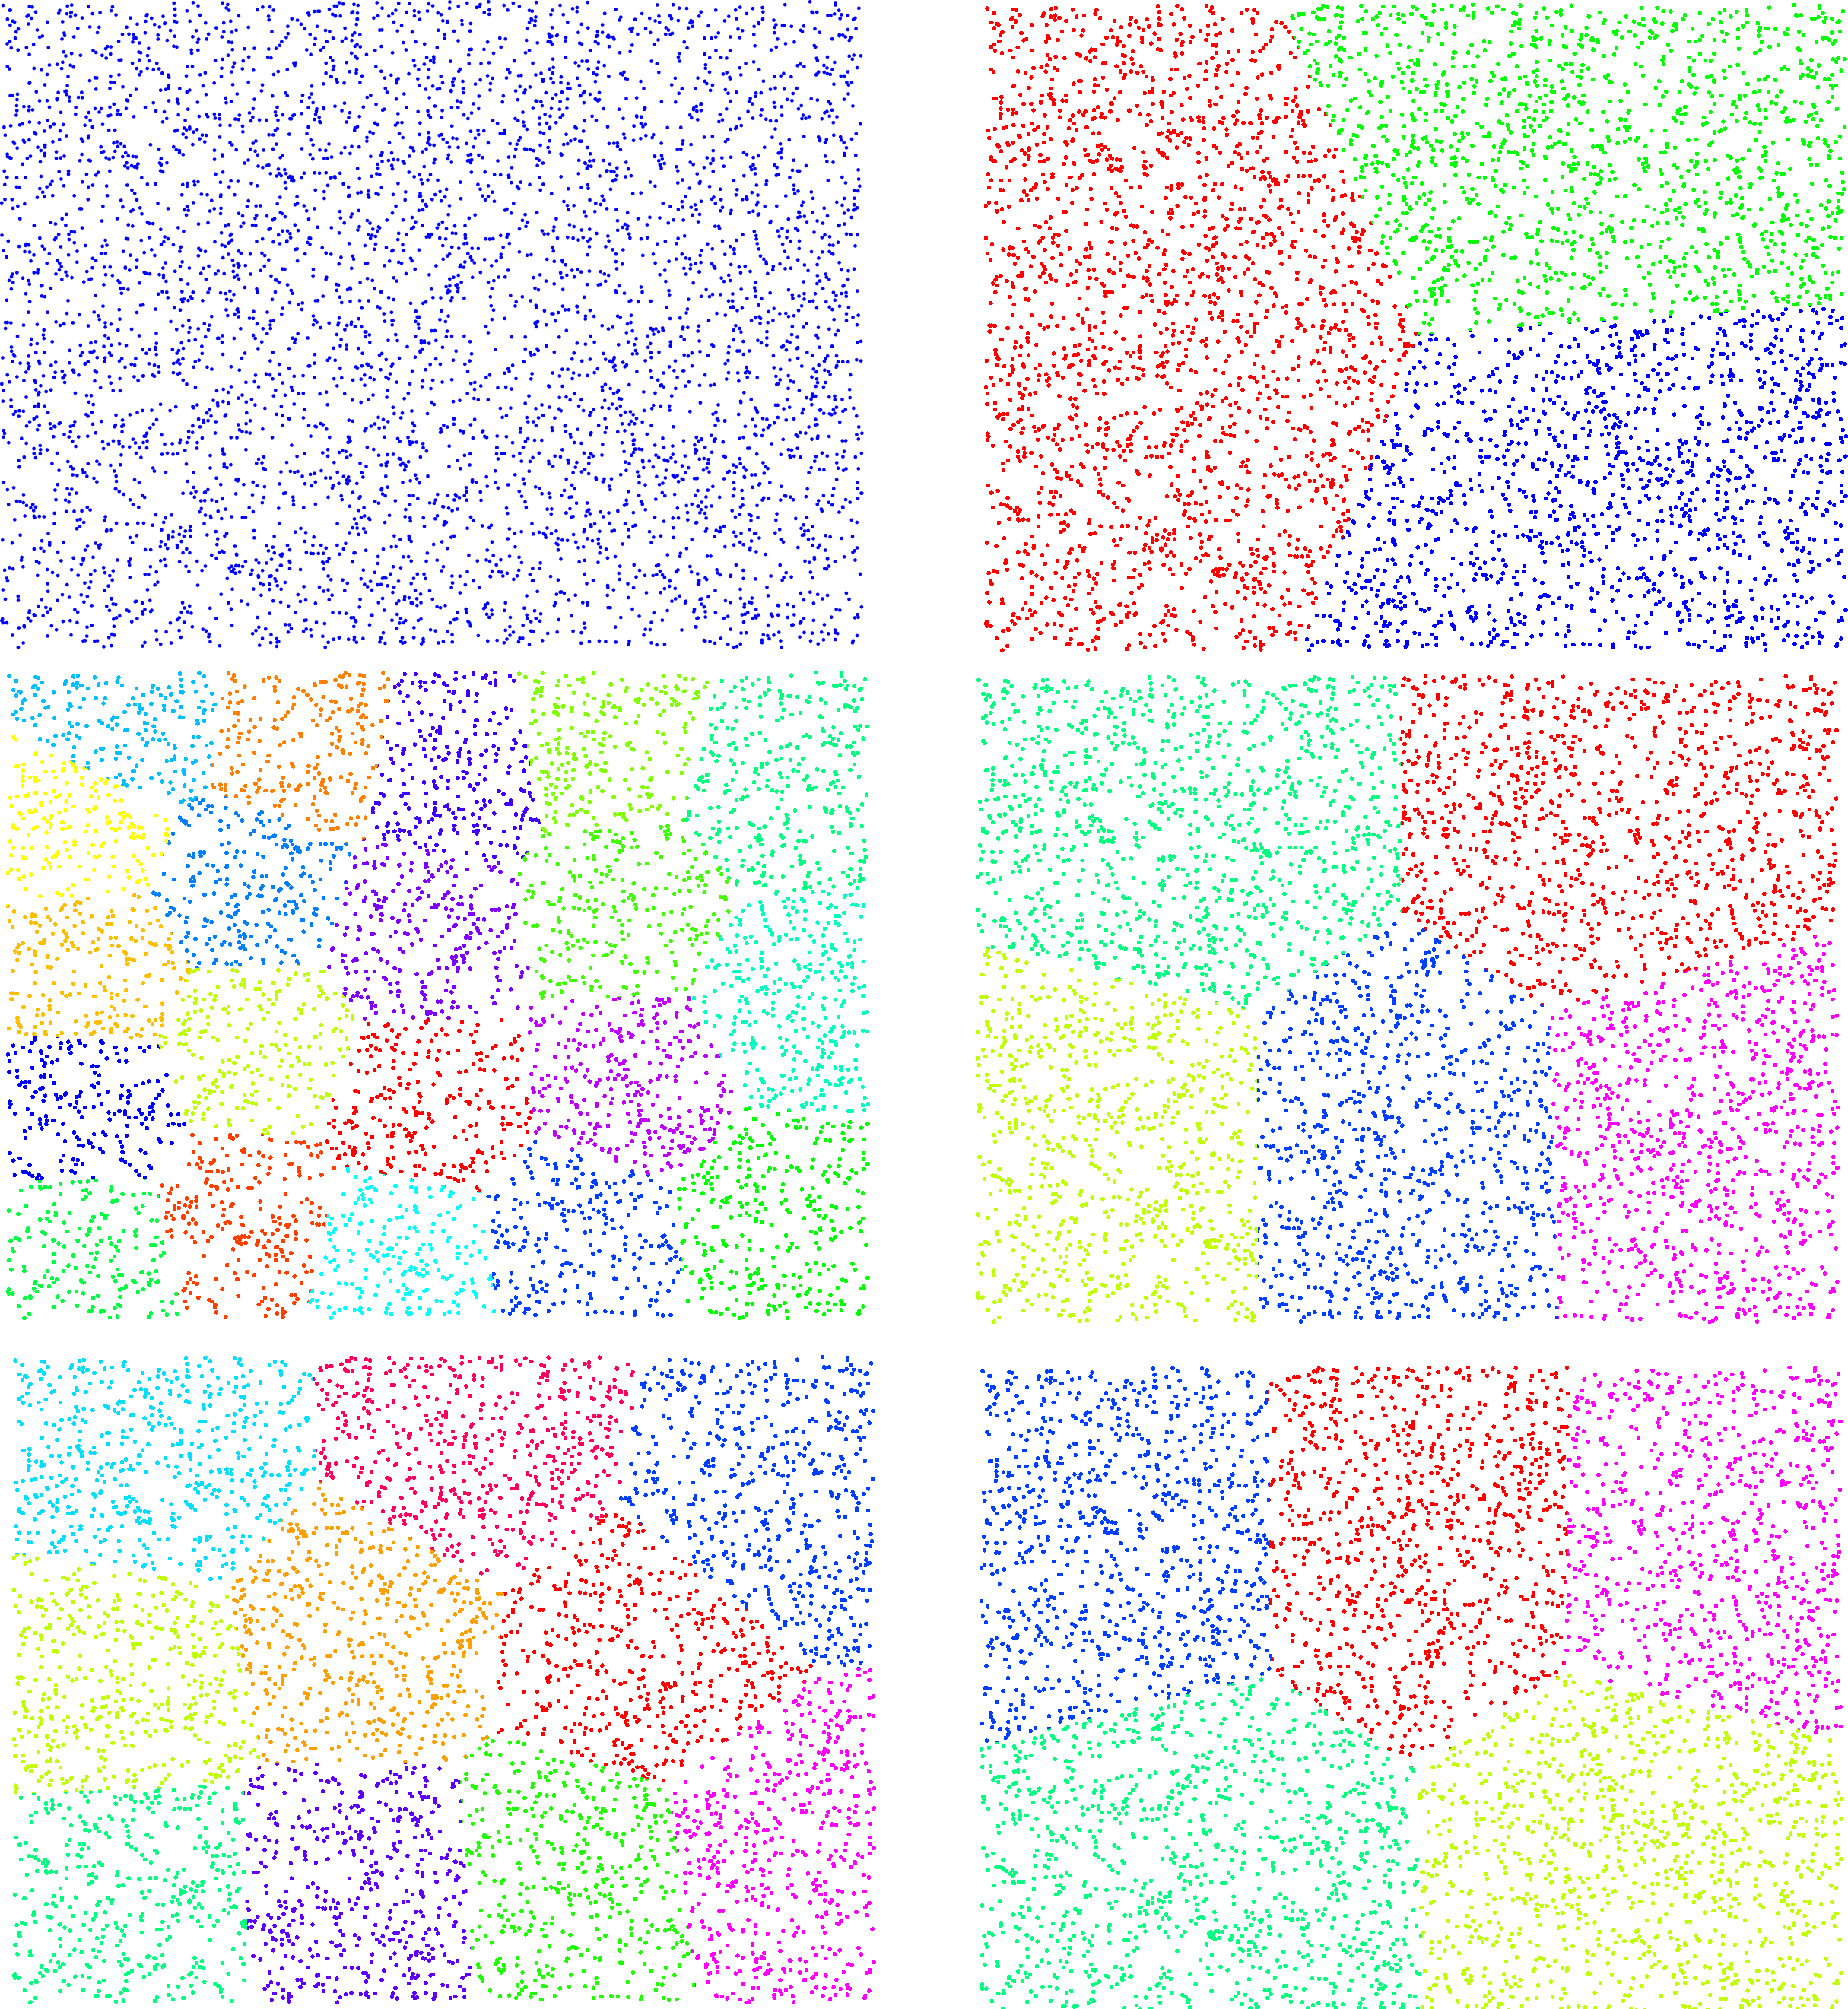
\includegraphics[width=0.5\textwidth]{./img/number.png}
	\caption{Od górnego lewego rogu zgodnie ze wskazówkami zegara: obraz oryginalny, k = 3, k = 5, k = 5, k = 10, k = 20}
	\label{img:number}
\end{figure}

Na rysunku nr \ref{img:number} przedstawiono wyniki wykonania algorytmu dla różnych liczby grup. Jako warunek stopu ustawiono stan stabilny. Algorytm zachowuje się poprawnie każdej liczby grup, jednak należy zwrócić uwagę, że dla identycznych parametrów wykonania (w tym przypadku k = 5) algorytm może zwrócić różne wyniki -- jest to efekt losowego doboru centroidów.

\subsubsection{Zależność od danych wejściowych}

\begin{figure}[!h]
	\centering
	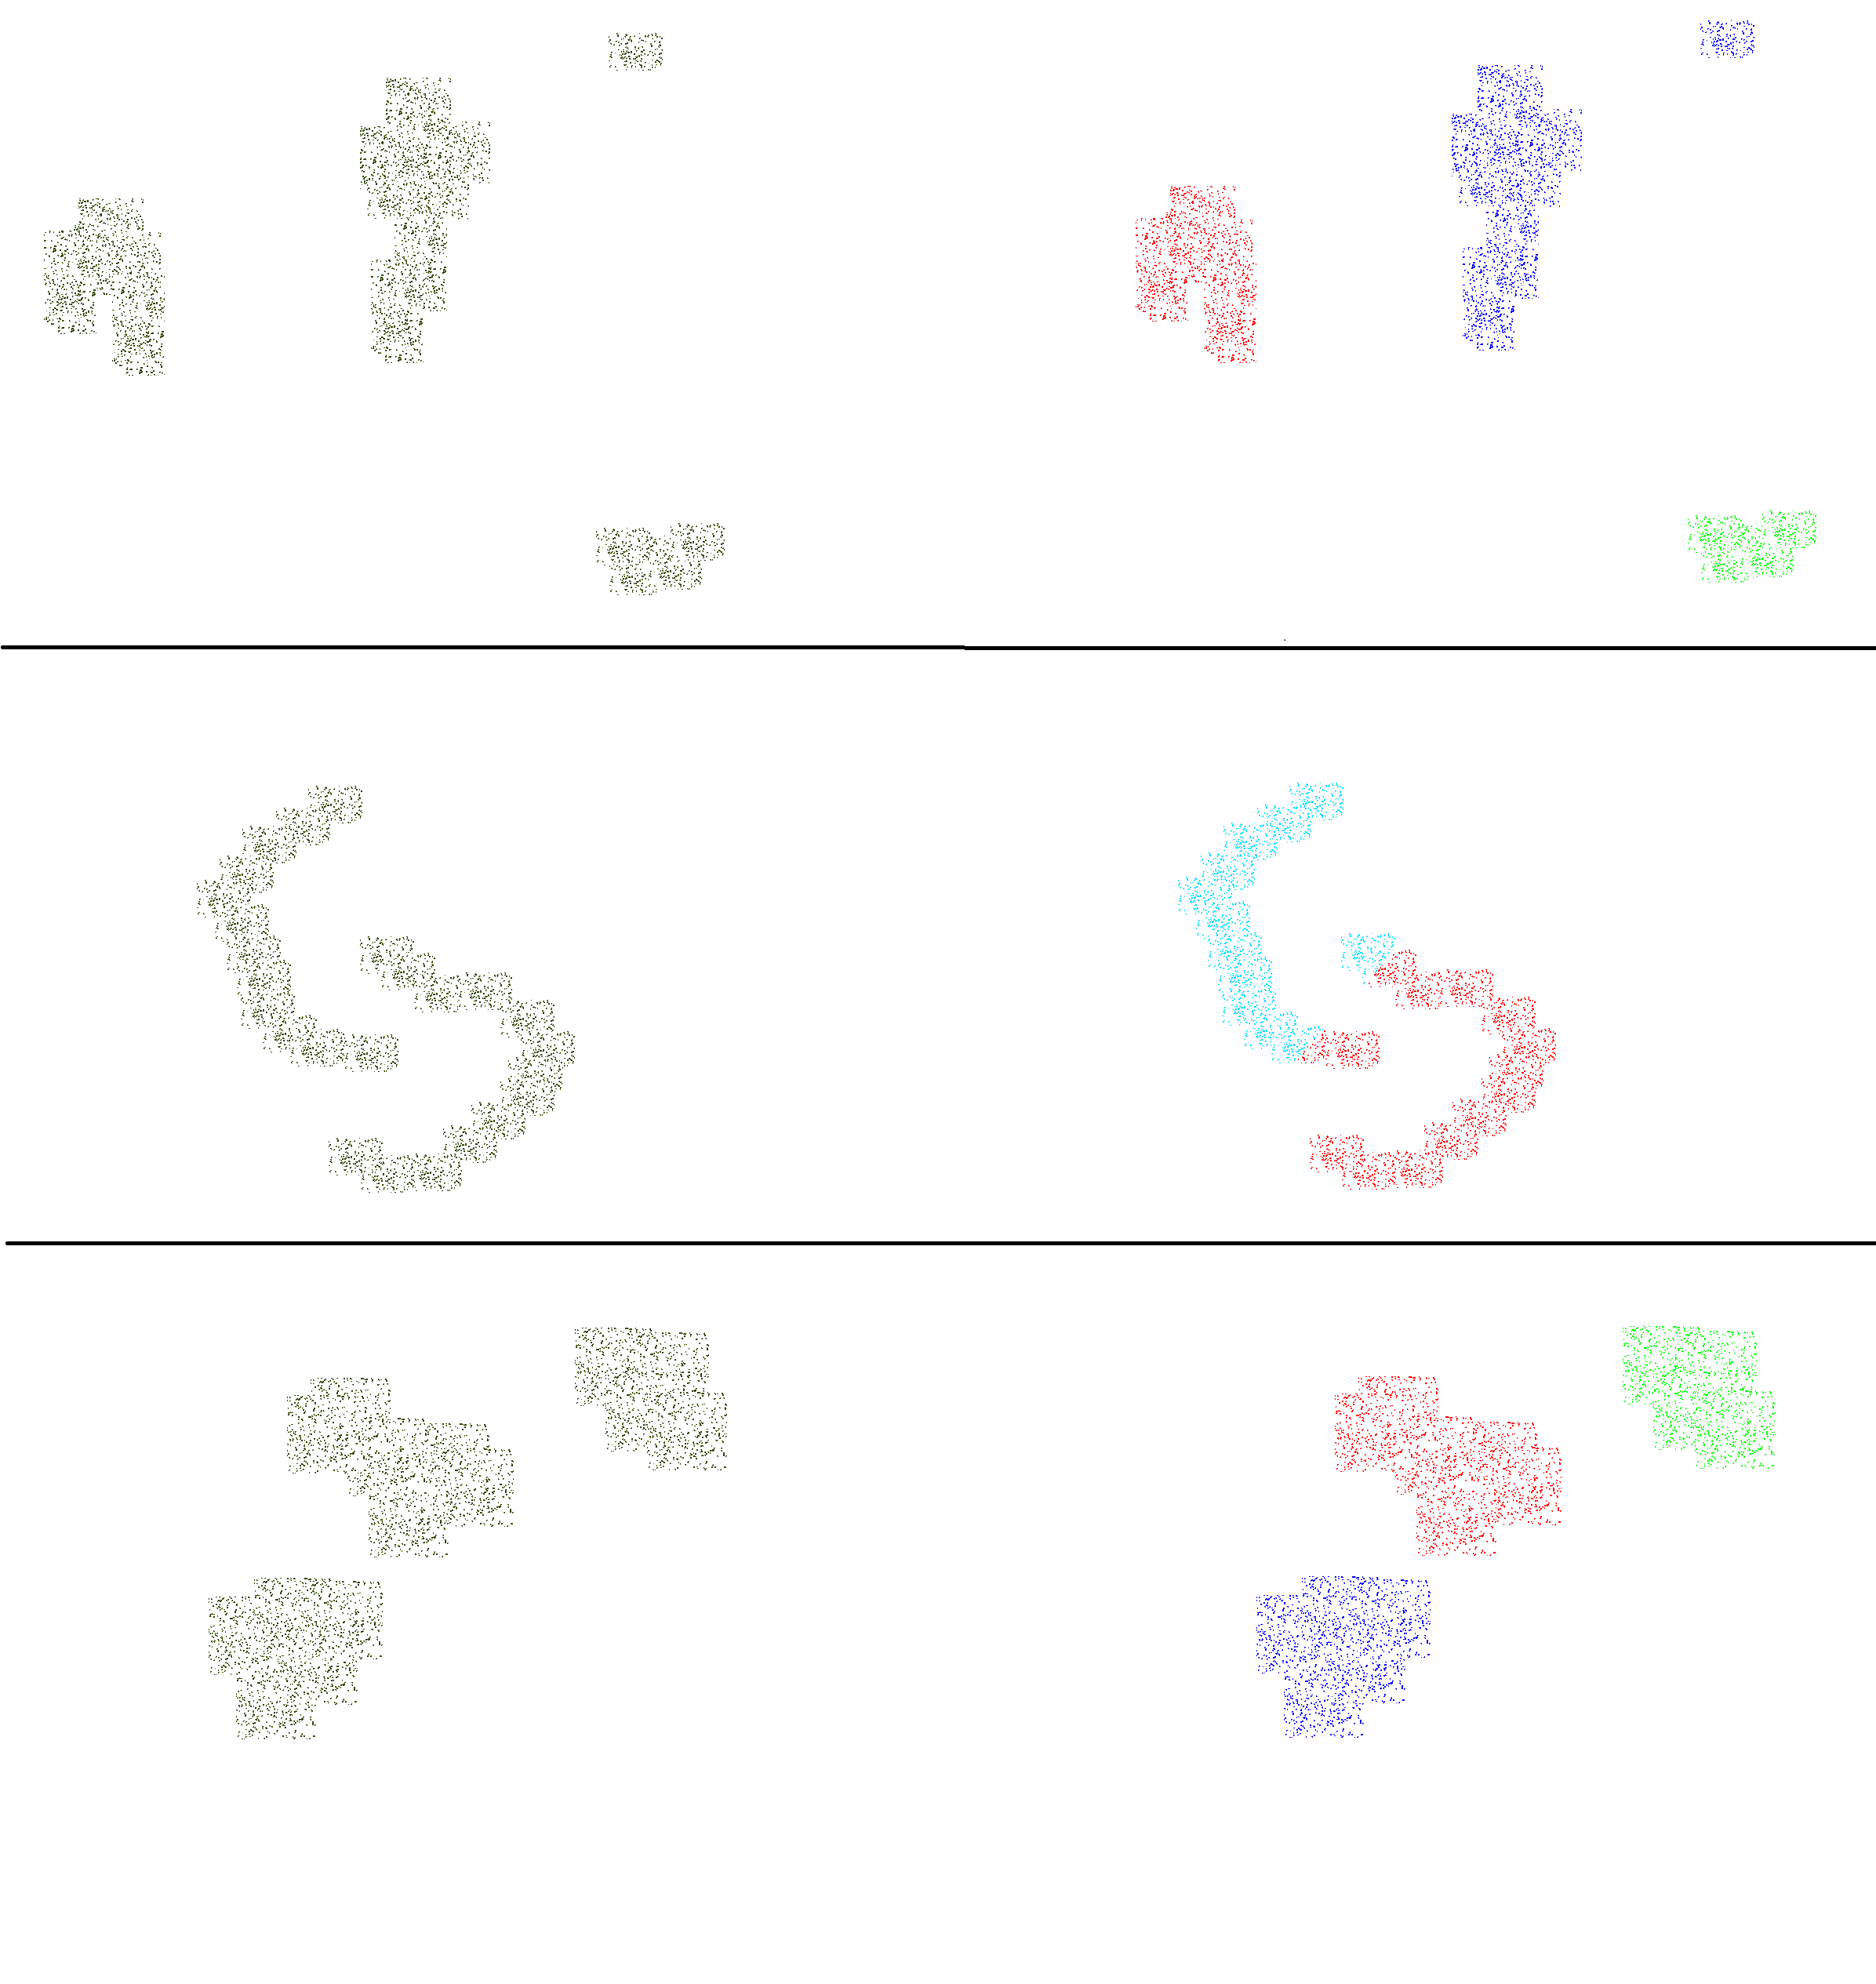
\includegraphics[width=0.6\textwidth]{./img/shape.png}
	\caption{Po lewej: obrazy przed grupowaniem, po prawej po grupowaniu}
	\label{img:shape}
\end{figure}

Na rysunku nr \ref{img:shape} przedstawiono wyniki wykonania algorytmu dla różnych kształtów bitmap. Jako warunek stopu ustawiono stan stabilny. Dla przykładów pierwszego i trzeciego algorytm sprawił się bardzo dobrze, grupując według wyraźnie oddzielonych grup (dla pierwszegho przykładu jeszcze lepsze wyniki możnaby otrzymać zwiększając liczbę grup do 4). Dla przykładu drugiego rozwiązanie nie jest do końca optymalne -- w tym przypadku lepsze mogłoby się okazać wykorzystanie innego algorytmu grupowania.